
\chapter{初期グラフの変更による探索空間の削減}
\label{chap:reduce-by-initial-graph}
\ref{sect:apply-to-gmg}節の定義\ref{def:basic-initial-graph}
で述べた基本初期グラフを変更することで探索空間を削減し,
探索を効率的に行う.本章では,新たに定義する二つの初期グラフについて,
その構築法と妥当性に関する予想を与え,変更の効果を実験により検証する.

\section{長さ$2Q+2$の閉路を含む初期グラフ}
\label{sect:initial-graph-cycle}
長さ$2Q+2$の閉路を含む初期グラフ$G_I$を次のように定義する.
ただし,このような初期グラフは$R(n,k)>0$を満たすときのみ構築できる.
\begin{definition}[長さ$2Q+2$の閉路を含む初期グラフ]
  \label{def:cycle-initial-graph}
  次のグラフ$G_I$を\textbf{閉路を含む初期グラフ}あるいは
  \textbf{閉路初期グラフ}と呼ぶ.ただし,$G_I'=(V',E')$を定義
  \ref{def:basic-initial-graph}の基本初期グラフとする.
  \begin{equation}
    \begin{aligned}
      G_I&=(V',E'\cup\{\{p,r\},\{q,r\}\}) \\
      p&=n_{k,\hat{Q}-2}+1 \\
      q&=n_{k,\hat{Q}-2}+1+(k-1)^{\hat{Q}-2} \\
      r&=n-R+1
    \end{aligned}
  \end{equation}
\end{definition}
閉路初期グラフの例として,$n=12$,$k=3$の閉路初期グラフの図を
図\ref{fig:initial-graph-cycle-example}に示す.

\begin{figure}
  \centering
  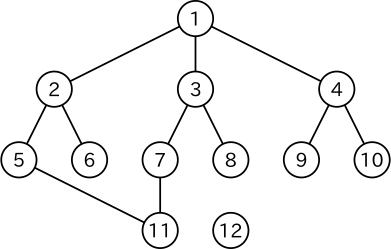
\includegraphics[width=.4\linewidth]{initial-tree-cycle-example.pdf}
  \caption{長さ6の閉路を含む,頂点数12,次数3の初期グラフ}
  \label{fig:initial-graph-cycle-example}
\end{figure}

定義\ref{def:cycle-initial-graph}で定義したグラフを初期グラフとすることの
妥当性はまだ証明されていない.それに関する予想を次の予想\ref{conj:gmg-cycle}
で与える.
\begin{conjecture}
  \label{conj:gmg-cycle}
  一般化ムーアグラフ$M(n,k)$には,長さ$2Q+2$の閉路が少なくとも一つ存在する.
  ただし,$R(n,k)>0$とする.
\end{conjecture}

\subsection*{候補辺の並べ替え}
閉路初期グラフから得られる候補辺は,頂点$v$に対する$\text{Enter}(v)$と
$\text{Exit}(v)$の値が大きくなるため,正則グラフであることの判定が遅くなり
探索が効率よく行えない.そこで,グラフの候補辺をアルゴリズム
\ref{algo:sort-edges}で述べる手順で並べ替える.
\begin{algorithm}[H]
  \caption{項補辺の並べ替え}
  \label{algo:sort-edges}
  \begin{algorithmic}[1]
    \Require $\{e_i\}_{i\in\mathbb{N}}^M$
    \Ensure 並べ替え後の候補辺$\{e'_i\}_{i\in\mathbb{N}}^M$
    \Procedure{SortCandidateEdges}{$\{e_i\}_{i\in\mathbb{N}}^M$}
    \State $V\gets e_1\cup e_2\cup\cdots\cup e_M$
    \Comment 頂点集合を得る
    \State $E\gets\{e_i\}$
    \State $E'\gets()$
    \While{$|E|>0$}
    \State $n_v\gets0\,(v\in V)$
    \ForAll{$\{v,w\}\in E$}
    \State $n_v\gets n_v+1,\,n_w\gets n_w+1$
    \EndFor
    \State $v\gets \argmax_v\{n_v\}$
    \State $F\gets \{e\,|\,v\in e,\,e\in E\}$
    \State $E'\gets E'F,\,E\gets E\setminus F$
    \Comment $E'$に追加,$E$から削除
    \EndWhile
    \EndProcedure
  \end{algorithmic}
\end{algorithm}

\section{全域木}
\label{sect:initial-spanning-tree}
初期グラフとしての全域木$G_I$を次の定義\ref{def:stree-initial-graph}で定義する.
\begin{definition}[初期グラフとしての全域木]
  \label{def:stree-initial-graph}
  頂点数$n$,次数$k$に対して,次の全域木$G_I$を
  \textbf{初期グラフとしての全域木}あるいは
  \textbf{全域木初期グラフ}と呼ぶ.
  \begin{equation}
    \begin{aligned}
      G_I&=(V,E) \\
      V&=\{1,\ldots,n\} \\
      E&=\{\{1,2\},\ldots,\{1,k+1\}\}\cup
      \{\{\text{parent}(v),v\}\,|\,v\in \{k+2,\ldots,n\}\}  \\
      \text{parent}(v)&=
      (v-n_{k,\hat{Q}(v)-1}-1)\mod(k(k-1)^{\hat{Q}(v)-2})+1+n_{k,\hat{Q}-1}
    \end{aligned}
  \end{equation}
  ここで,$\mod$は除余を表す.
\end{definition}
全域木初期グラフの例として,$n=12$,$k=3$と$n=18$,$k=3$の二つの
全域木初期グラフの図を図\ref{fig:initial-spanning-tree-example}に
示す.

\begin{figure}
  \centering
  \subfloat[頂点数$12$,次数$3$の全域木]{
    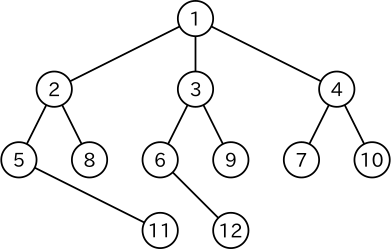
\includegraphics[width=.4\linewidth]
                    {initial-spanning-tree-12-example.pdf}
  }\hfill
  \subfloat[頂点数$18$,次数$3$の全域木]{
    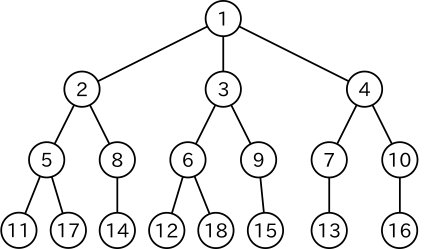
\includegraphics[width=.45\linewidth]
                    {initial-spanning-tree-18-example.pdf}
  }
  \caption{全域木の例}
  \label{fig:initial-spanning-tree-example}
\end{figure}

定義\ref{def:stree-initial-graph}で定義された初期グラフから探索することの
妥当性は証明されていない.次の予想\ref{conj:spanning-tree}はその妥当性に関する
予想である.
\begin{conjecture}
  \label{conj:spanning-tree}
  一般化ムーアグラフ$M(n,k)$の全域木に,定義\ref{def:stree-initial-graph}
  で定義された木が存在する.
\end{conjecture}
また,条件を緩めて次のことも予想される.
\begin{conjecture}
  \label{conj:spanning-tree-2}
  一般化ムーアグラフ$M(n,k)$の全域木に,次の性質を満たす木が存在する.
  \begin{itemize}
  \item ある頂点$v$とのの距離が$Q$である頂点集合$V=\{w\,|\,d(v,w)=Q\}$に
    ついて,次が成り立つ. \\
    \[ \max\{d(w)\,|\,w\in V\}-\min\{d(w)\,|\,w\in V\}\leq 1 \]
    つまり,次数の差がたかだか1である.
  \end{itemize}
\end{conjecture}

\section{実験}
\label{sect:exp-reduce-by-initial}
提案した初期グラフの有効性を検証するため,実験を行う.
初期グラフを変更するには,定義\ref{def:basic-initial-graph}の基本初期グラフを
定義\ref{def:cycle-initial-graph}(閉路初期グラフ)や
定義\ref{def:stree-initial-graph}(全域木初期グラフ)に置き換えればよい.
なお,実験で測定する項目やパラメータ,実験環境は
\ref{sect:exp-basic-algorithm}節に示したものと同じである.

\section{結果}
\label{sect:result-reduce-by-initial}
探索開始から最初の一般化ムーアグラフの発見までに要した探索時間を
図\ref{fig:ginitr-time}に示す.探索開始から最初の一般化ムーアグラフの発見までの
状態展開数を図\ref{fig:ginitr-state}に示す.さらに,一般化ムーアグラフの列挙で
取り出されたグラフ数を図\ref{fig:ginitr-ngraph}に示す.

図\ref{fig:ginitr-time}と図\ref{fig:ginitr-state}より,
全域木から探索を開始すれば最速かつ最も展開状態数が少ないことが分かる.
また,同じ図より,閉路を含む初期グラフにおいて,アルゴリズム
\ref{algo:sort-edges}に示した候補辺の並べ替えを行うことで,
頂点数が比較的大きい場合に高速化と高効率化ができていることが分かる.

図\ref{fig:ginitr-ngraph}より,多くの頂点数と次数の組$(n,k)$に対して,
全域木から探索する場合が最も総グラフ数が少ない.これは,全域木の候補辺が
他の初期グラフの候補辺より少なくなっているためと考えられる.しかし,
$R=2\,((n,k)=(6,3),(12,3),(7,4))$の組合せに対しては,閉路初期グラフの
総グラフ数が最小である.
なお,一般化ムーアグラフの列挙は,候補辺の並べ替えによる影響がないことに
注意する.なぜなら,列挙は候補辺に含まれる辺のすべての組み合わせの中から,
一般化ムーアグラフを生じるものを抜き出すためである.

\begin{figure}
  \centering
  \noindent\makebox[\textwidth]{
    \includegraphics{ginitr-time-lpad.pdf}
    \includegraphics{ginitr-time-ylab.pdf}
    \includegraphics{ginitr-time-d3-yaxis.pdf}\hspace{-3mm}
    \subfloat[$k=3$]{
      \includegraphics{ginitr-time-d3.pdf}
    }\hspace{5mm}
    \includegraphics{ginitr-time-d4-yaxis.pdf}\hspace{-3mm}
    \subfloat[$k=4$]{
      \includegraphics{ginitr-time-d4.pdf}
    }
    \includegraphics{ginitr-time-legend.pdf}
  }
  \caption{最初の一般化ムーアグラフの発見までの時間}
  \label{fig:ginitr-time}
\end{figure}

\begin{figure}
  \centering
  \noindent\makebox[\textwidth]{
    \includegraphics{ginitr-state-lpad.pdf}
    \includegraphics{ginitr-state-ylab.pdf}
    \includegraphics{ginitr-state-d3-yaxis.pdf}\hspace{-3mm}
    \subfloat[$k=3$]{
      \includegraphics{ginitr-state-d3.pdf}
    }\hspace{5mm}
    \includegraphics{ginitr-state-d4-yaxis.pdf}\hspace{-3mm}
    \subfloat[$k=4$]{
      \includegraphics{ginitr-state-d4.pdf}
    }
    \includegraphics{ginitr-state-legend.pdf}
  }
  \caption{最初の一般化ムーアグラフの発見までの展開状態数}
  \label{fig:ginitr-state}
\end{figure}

\begin{figure}
  \centering
  \noindent\makebox[\textwidth]{
    \includegraphics{ginitr-ngraph-lpad.pdf}
    \includegraphics{ginitr-ngraph-ylab.pdf}
    \includegraphics{ginitr-ngraph-d3-yaxis.pdf}\hspace{-3mm}
    \subfloat[$k=3$]{
      \includegraphics{ginitr-ngraph-d3.pdf}
    }\hspace{5mm}
    \includegraphics{ginitr-ngraph-d4-yaxis.pdf}\hspace{-3mm}
    \subfloat[$k=4$]{
      \includegraphics{ginitr-ngraph-d4.pdf}
    }
    \includegraphics{ginitr-ngraph-legend.pdf}
  }
  \caption{列挙された一般化ムーアグラフの数}
  \label{fig:ginitr-ngraph}
\end{figure}
